\documentclass[conference, letterpaper, 11pt]{IEEEtran}

\IEEEoverridecommandlockouts
% The preceding line is only needed to identify funding in the first footnote. If that is unneeded, please comment it out.

\usepackage[style=ieee]{biblatex}
\usepackage{hyperref}
\usepackage{amsmath,amssymb,amsfonts}
\usepackage{algorithmic}
\usepackage{graphicx}
\usepackage{textcomp}
\usepackage{xcolor}
\usepackage{censor}

\usepackage{lipsum}

% \StopCensoring
\addbibresource{report.bib}

\begin{document}

\title{Visualizing Facebook Data
\thanks{Do we have a "funding source" to acknowledge?}
}

\author{\IEEEauthorblockN{Noah Duggan Erickson}
\IEEEauthorblockA{\textit{Dept. of Computer Science} \\
\textit{Western Washington University}\\
Bellingham, WA, USA \\
\censor{EMAIL REDACTED}}
\and
\IEEEauthorblockN{Peter Hafner}
\IEEEauthorblockA{\textit{Dept. of Computer Science} \\
\textit{Western Washington University}\\
Bellingham, WA, USA \\
\censor{EMAIL REDACTED}}
\and
\IEEEauthorblockN{Carter Jacobs}
\IEEEauthorblockA{\textit{Dept. of Computer Science} \\
\textit{Western Washington University}\\
Bellingham, WA, USA \\
\censor{EMAIL REDACTED}}
\and
\IEEEauthorblockN{Trevor Le}
\IEEEauthorblockA{\textit{Dept. of Computer Science} \\
\textit{Western Washington University}\\
Bellingham, WA, USA \\
\censor{EMAIL REDACTED}}
\and
\IEEEauthorblockN{Dustin O'Hara}
\IEEEauthorblockA{\textit{Dept. of Computer Science} \\
\textit{Western Washington University}\\
Bellingham, WA, USA \\
oharad@wwu.edu}
% \and
% \IEEEauthorblockN{6\textsuperscript{th} Given Name Surname}
% \IEEEauthorblockA{\textit{dept. name of organization (of Aff.)} \\
% \textit{name of organization (of Aff.)}\\
% City, Country \\
% email address}
}

\maketitle

\begin{abstract}
This is the abstract for our report. \lipsum[][1-5]
\end{abstract}

\begin{IEEEkeywords}
Facebook, Data Visualization, Social Media, Big Data
\end{IEEEkeywords}

\section{Introduction} \label{IN}

The goal for our project was to create a consumer-grade application for Facebook Users to easily interpret the data that Facebook has collected on them. We did this by creating an application that takes the user's data, in json format, and creates visualizations to give the user a greater understanding and in depth insight of their data. From our client, Dustin O'hara, we were instructed to implement a story-like format when creating our visuals so that users who view their own data apply their own interpretation. To establish the final scope of the project, we finalized on the idea of having our visualizations implemented onto a website where users can view our findings and the comparisons of us as Facebook users. The website will be implemented by Carter Jacobs and if the users are interested they are about to download a package which allows them to implement their own Facebook Profile data and view their own visuals. 

Our project was only made possible from the General data Protection Regulation (GDPR) forcing companies to allow the users to view, edit and delete the data collected on them. The motivation behind this project was powered by the want of unraveling the contents of Facebook's data collection. We wanted users of all ages and skill levels to be able to make sense of the data. 

The collection of our hard work will provide opportunities for education of one's digital footprint and spread awareness on the mysteries on how Facebook or companies similar to Facebook collect data on their users. 

\section{Related Work} \label{RW}

With the ubiquity of social media platforms in the modern age~\cite{metapress}, it is no surprise that these monolithic services collect/hold unfathomable quantities of data on their users. This data can then be used by Meta and their advertising partners to infer a user's interests, preferences, and behaviors. However, these inferences can frequently be made erroneously or in ways that do not align with the user's true self or values.

A prime example of where these discrepancies can manifest lies in the algorithmic profiling for ads interests, which \cite{algprof} found to at least “somewhat accurate[ly]” reflect the user in only 47.6\% of survey participants. On the other hand, textual data such as posts, comments, and messages can be used in a variety of ways, including in depression detection, where \cite{depression} shows an F1 score (see Eqn.~\ref{eqn:f1}) of 0.89 on a Twitter-based dataset.

\begin{equation}
    F1 = \frac{2 \cdot P \cdot R}{P + R}\label{eqn:f1}
\end{equation}

Where divides occur, they manifest from a variety of sources such as the difficulty of retrospective geolocation of IPv4 addresses~\cite{ipgeo}, and the false persona we present while online~\cite{fbself}. This "garbage in, garbage out" phenomenon highlights the inherent challenges in deriving accurate insights from social media data, as the input data may be inherently flawed or misleading.

Despite these shortcomings, much of the literature approaches user-centric Facebook data analysis with the intent to surprise the user about the sheer quantity of data, without considering the quality thereof~\cite{surpriv, usercontext}. In this project, we aim to take a different approach - one that centers on digital self-reflection by encouraging users to interact with their data in a way that motivates and self-generates individual discovery and insight.

\section{Methodology} \label{ME}

We focused on making sure that all the visualizations that we created were going to have some meaning behind them. We looked at all the files to find files that we found the most interesting. Our final selection of files includes all the messaging files, topics, (SPECIFIC FILE NAMES HERE). We also wanted to provide the user with an overall interactive view of the size of their data, as each individual user’s data has differing sizes from a few megabytes to several gigabytes. 

We created six main methods, one for each type of visualization we decided to use. There is Facebook activity, off Facebook activity, filesize sunburst, location via IP addresses, notification charting, and interests. Each creating unique and in-depth visualizations on their respective files. There are two groups of methods that we have, there are three word based methods and three statistical methods. The word based methods are on and off facebook activity and interests and the statistical methods are filesize sunburst, location via IP addresses, and notification charting. 

Going more in depth, the word based methods are focused on the words that are contained inside the files, rather than specific numeric values in the files. Facebook activity uses the users messaging data to create sentiment plots along with word clouds of the users most messaged words over time. Off Facebook activity uses what other sites report to Facebook that the user has visited and creates a visual showing the top 5 most visited sites and all sites the user has visited over 50 times. Interests takes the data of what ads the user is interested in and creates a collage of pictures of those interests to show the user the variety that Facebook thinks they are interested in.

The statistical methods use the numerics of the data to give the user more insight. Filesize sunburst uses all the users data files and creates a sunburst showing the size of each folder in comparison to all the other folders. That includes an interactable site that allows the user to click on folders to enhance the composition of that folder. Location via IP addresses takes all the IP addresses that Facebook collects from the user and creates a map showing all the specific locations and how many times the user has been tracked at that location. Notification charting uses the past 30 days(the amount of days that Facebook holds onto this type of data per user) of notifications that a user has received and plots them in a similar manner to the github contributions graph.

All of the methods use a variety of Python libraries, ranging from Pandas to beautifulsoup4 to matplotlib. (IM NOT SURE WHAT ELSE TO ADD HERE, IF ANYTHING)

\section{Results \& Analysis} \label{RA}
\textbf{This is Peter's Results section.} \lipsum[1]

\textbf{An example of how to include a figure is shown in Fig.~\ref{fig:xmp}.} \lipsum[1]

\begin{figure}[htbp]
    \centerline{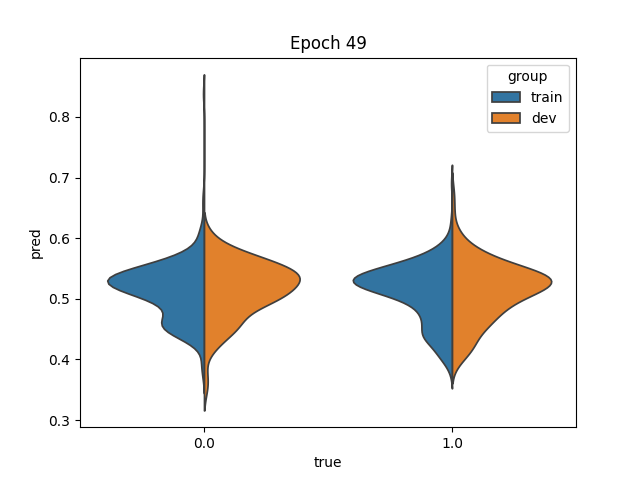
\includegraphics[width=3in]{img/3-1e49violin.png}}
    \caption{ABIDE CNN Model predictions at epoch 49 from \cite{aiad}.}
    \label{fig:xmp}
\end{figure}

\textbf{Even more figures are shown in Fig.~\ref{fig:xmp2}.} \lipsum[1]

\begin{figure}[htbp]
    \centerline{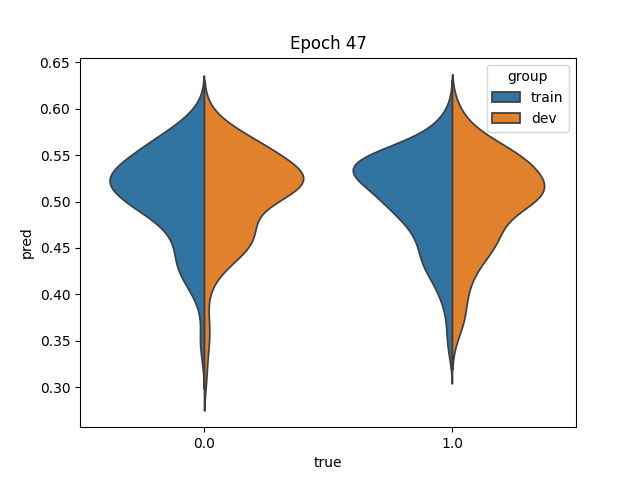
\includegraphics[width=3in]{img/3-1e47violin.png}}
    \centerline{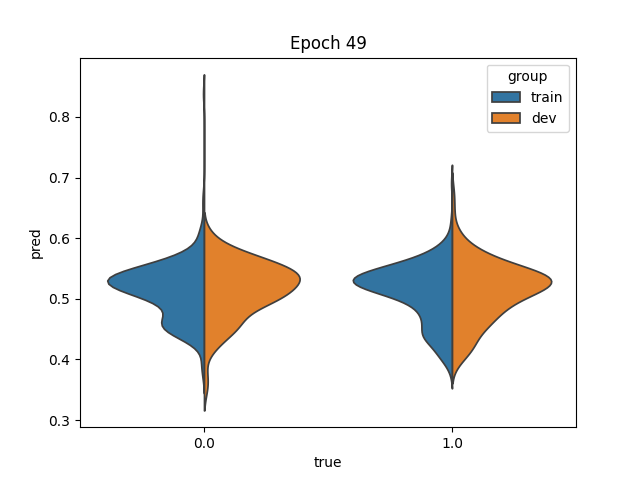
\includegraphics[width=3in]{img/3-1e49violin.png}}
    \caption{ABIDE CNN Model predictions at multiple epochs from \cite{aiad}.}
    \label{fig:xmp2}
\end{figure}

\textbf{An example of how to include a table is shown in Table~\ref{tab:xmp}.} \lipsum[1]

\begin{table}[htbp]
    \caption{Pointless table.}
    \begin{center}
        \begin{tabular}{|c|c|c|}
            \hline
            \textbf{C1} & \textbf{C2} & \textbf{C3} \\
            \hline
            1 & 2 & 3 \\
            4 & 5 & 6 \\
            7 & 8 & 9 \\
            \hline
        \end{tabular}
    \end{center}
    \label{tab:xmp}
\end{table}

\colorbox{red}{\color{white}{\textbf{NOTE: Positioning of the figs/tables known-bad -}}}
\colorbox{red}{\color{white}{\textbf{Will be refined when actual content is available.}}}

\lipsum[1-10]

\section{Conclusion} \label{CO}
\textbf{This is Trevor's Conclusion section.} \lipsum[1-2]

\section*{Acknowledgments}

Among others, we would like to thank Dr. Brian Hutchinson and Piper Wolters for their guidance and support throughout this project. \lipsum[][1-2]

\printbibliography
\end{document}
